\chapter{Validación sobre el panel de diez activos}
\label{cap:panel}

% Fuente única de cifras: notebooks/STRATA_marco_practico.ipynb (panel canónico de 10) y sus JSON en
% outputs/experiments/. Toda cifra trazada a su JSON en el caption de su tabla.

En SPY STRATA rescató al agente, pero sobre un único activo el intervalo de confianza del $\Delta$Sharpe del rescate cruzaba el cero: la corrección apuntaba bien, mas no se separaba del cero en solitario. La prueba dura vive en el panel: diez activos (SPY, QQQ, XLF, DIA, XLK, XLE, ROKU, SMCI, MARA, UNG), elegidos por su naturaleza para cubrir distintos grados de \emph{leverage effect}. Sobre ellos repetimos toda la cadena de SPY, agregamos los resultados y buscamos el patrón que ordena el rescate. Al apilar el panel, el rescate de riesgo que en un activo no alcanzaba significancia la alcanza.

\section{El rescate en el panel}
\label{sec:panel-agregado}

El problema que vimos en SPY no es de SPY. A través del panel el agente pierde y acierta menos de la mitad de las direcciones con regularidad: queda por debajo de $0{,}5$ en siete de los diez activos, y allí donde lo supera lo hace por poco y con un Sharpe pobre. El agente solo no es una estrategia, es el punto de partida que STRATA tiene que corregir.

\subsection{La compuerta de régimen y la activación de detectores}
\label{sec:panel-gate}

Los tres detectores no se encienden por igual. RAM domina en todas partes, igual que en SPY; PSA y GSO disparan poco, porque el agente mantiene posiciones casi constantes y sus \emph{scores} rara vez cruzan los umbrales. La Tabla~\ref{tab:mp-gate} recoge la tasa de intervención por activo y la compuerta de régimen: en los días en que RAM dispara, seguir el signo del régimen bate a seguir al agente en \textbf{seis de los diez} activos. La intervención no se reparte al azar: su tasa crece con la discrepancia entre la apuesta del agente y el signo del régimen, y esa relación es casi recta (Figura~\ref{fig:mp-gate-ram}; activo a activo en la Figura~\ref{fig:mp-activacion-panel} del Anexo~\ref{anx:figuras}).

\begin{table}[htbp]
\centering
\caption{Activación de RAM y compuerta de régimen por activo (OOS completo del panel). ``Tasa interv.'' es la fracción de días en que RAM dispara; ``discrepancia'' es la fracción de días en que la apuesta del agente choca con el signo del régimen; ``gate RAM'' indica si, en los días de disparo, seguir el régimen bate a seguir al agente. PSA y GSO disparan de forma marginal en todo el panel.}
\label{tab:mp-gate}
\begin{tabular}{lrrl}
\toprule
Activo & Tasa interv.\ (RAM) & Discrepancia agente$\leftrightarrow$régimen & Gate RAM \\
\midrule
SPY  & $0{,}302$ & $0{,}601$ & régimen $>$ agente \\
QQQ  & $0{,}197$ & $0{,}526$ & régimen $>$ agente \\
XLF  & $0{,}549$ & $0{,}720$ & régimen $>$ agente \\
DIA  & $0{,}343$ & $0{,}603$ & agente $>$ régimen \\
XLK  & $0{,}095$ & $0{,}372$ & agente $>$ régimen \\
XLE  & $0{,}596$ & $0{,}781$ & régimen $>$ agente \\
ROKU & $0{,}710$ & $0{,}823$ & régimen $>$ agente \\
SMCI & $0{,}018$ & $0{,}120$ & régimen $>$ agente \\
MARA & $0{,}415$ & $0{,}666$ & agente $>$ régimen \\
UNG  & $0{,}078$ & $0{,}169$ & agente $>$ régimen \\
\bottomrule
\end{tabular}
\end{table}

\begin{figure}[htbp]
\centering
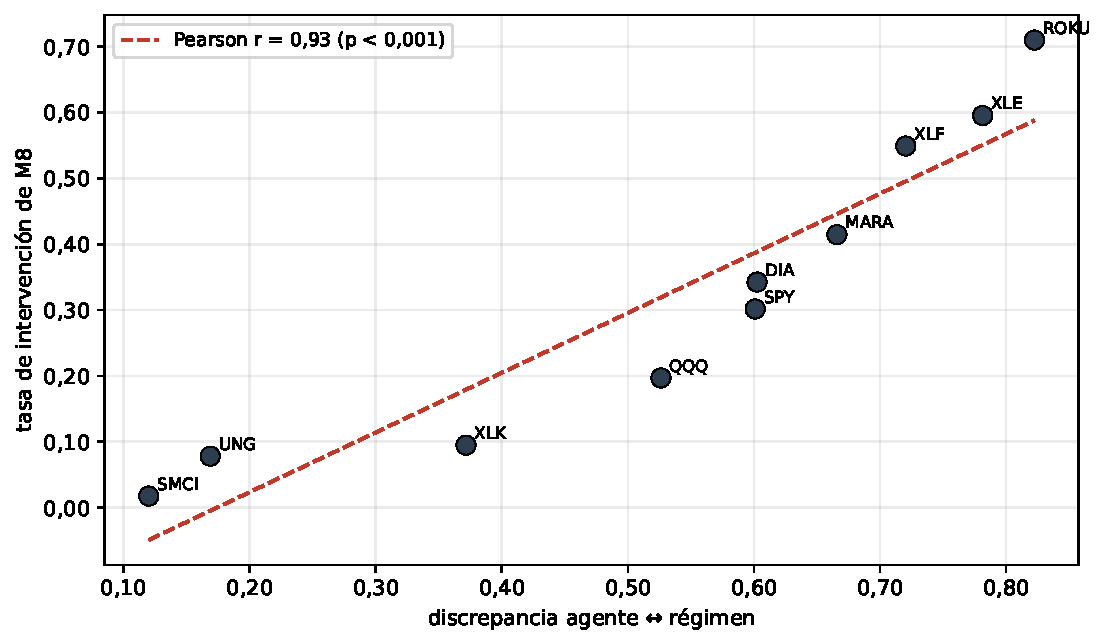
\includegraphics[width=0.60\textwidth]{figuras/cap4_gate_ram}
\caption{Compuerta de régimen sobre el panel: tasa de intervención de RAM frente a la discrepancia media entre la apuesta del agente y el signo del régimen, un punto por activo. La relación es casi recta (Pearson $r = 0{,}93$, $p < 0{,}001$): cuanto más se aleja el agente del estado del mercado, con más frecuencia actúa la regla.}
\label{fig:mp-gate-ram}
\end{figure}

\subsection{Accuracy por activo: dónde se bate a la trivial}
\label{sec:panel-accuracy}

La Tabla~\ref{tab:mp-accuracy} cruza los diez activos con las seis estrategias en accuracy direccional. La mejor derivada de STRATA mejora al agente en los \textbf{diez de diez} activos, con una mejora media de $+0{,}086$; en ninguno supervisar lo empeora. Qué estrategia gana cambia de un activo a otro, coherente con la idea de dos capas: en unos manda la regla, en otros el aprendiz, según la naturaleza del activo.

\begin{table}[htbp]
\centering
\caption{Accuracy direccional por activo y estrategia (ventana desplegable, \texttt{signal\_lag}${}=1$). En negrita, la mejor derivada de STRATA (M8/M10/AutoML) cuando supera a las dos referencias triviales (ZeroR y B\&H) en ese activo. ZeroR y B\&H comparten valor salvo cuando difieren.}
\label{tab:mp-accuracy}
\begin{tabular}{lrrrrrr}
\toprule
Activo & M5 & M8 & M10 & AutoML & ZeroR & B\&H \\
\midrule
SPY  & $0{,}366$ & $0{,}442$ & $0{,}494$ & $\mathbf{0{,}574}$ & $0{,}566$ & $0{,}566$ \\
QQQ  & $0{,}418$ & $0{,}486$ & $0{,}522$ & $0{,}534$ & $0{,}590$ & $0{,}590$ \\
XLF  & $0{,}429$ & $0{,}502$ & $0{,}526$ & $0{,}510$ & $0{,}538$ & $0{,}538$ \\
DIA  & $0{,}440$ & $0{,}484$ & $0{,}468$ & $0{,}520$ & $0{,}552$ & $0{,}556$ \\
XLK  & $0{,}510$ & $0{,}470$ & $0{,}542$ & $0{,}590$ & $0{,}641$ & $0{,}641$ \\
XLE  & $0{,}448$ & $0{,}528$ & $0{,}508$ & $0{,}532$ & $0{,}565$ & $0{,}565$ \\
ROKU & $0{,}444$ & $0{,}528$ & $0{,}508$ & $0{,}544$ & $0{,}548$ & $0{,}548$ \\
SMCI & $0{,}484$ & $0{,}496$ & $\mathbf{0{,}552}$ & $0{,}472$ & $0{,}516$ & $0{,}484$ \\
MARA & $0{,}528$ & $0{,}528$ & $0{,}532$ & $\mathbf{0{,}544}$ & $0{,}532$ & $0{,}468$ \\
UNG  & $0{,}510$ & $0{,}502$ & $\mathbf{0{,}518}$ & $0{,}482$ & $0{,}449$ & $0{,}486$ \\
\bottomrule
\end{tabular}
\end{table}

En cuatro activos una derivada de STRATA supera en punto a las dos referencias triviales a la vez: SPY y MARA por AutoML, SMCI y UNG por M10 (Tabla~\ref{tab:mp-accuracy}, celdas en negrita). En los seis restantes la trivial aguanta; en índices muy direccionales como XLK la clase mayoritaria del pasado se va por encima de $0{,}64$ y ninguna derivada se le acerca.

Estas victorias son reales en punto y nominales. Con del orden de doscientos cincuenta días por activo y una ganadora que cambia de un activo a otro, se eligen a posteriori, y ninguna bate a ZeroR con significancia: el McNemar pareado de AutoML frente a ZeroR sobre SPY da $p = 0{,}90$, sin potencia para separarlos. El mapa completo está en la Figura~\ref{fig:mp-heatmap}, con solo cuatro celdas de derivada del lado bueno, y el reparto de aciertos y fallos en la Figura~\ref{fig:anx-confusion-panel}. La prueba que sí sobrevive a un test vive en el riesgo, no en la accuracy frente a la trivial.

\begin{figure}[htbp]
\centering
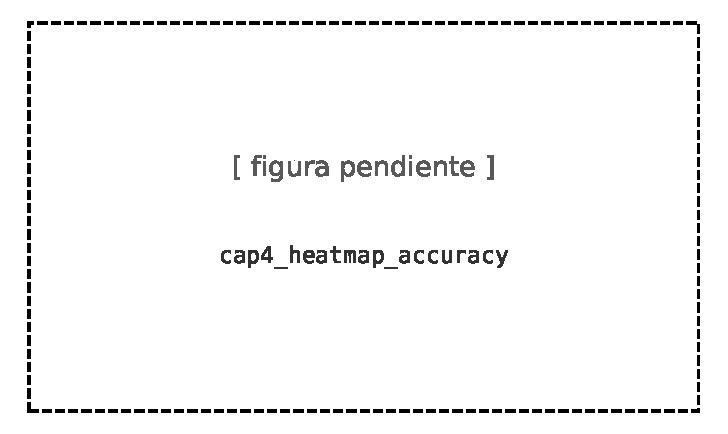
\includegraphics[width=0.62\textwidth]{figuras/cap4_heatmap_accuracy}
\caption{Mapa de calor de la accuracy direccional por activo (filas) y estrategia (columnas), centrado en $0{,}5$: el color mide la distancia a una referencia trivial. Verde marca accuracy por encima de la trivial del activo, rojo por debajo. La mejor derivada de STRATA supera a las dos triviales solo en SPY, SMCI, MARA y UNG; en los demás la trivial aguanta. Victorias nominales (n${}\approx 250$, a posteriori).}
\label{fig:mp-heatmap}
\end{figure}

\subsection{Pooled: el rescate en riesgo}
\label{sec:panel-pooled}

SPY mostró que el problema era de potencia, no de señal: con una muestra tan pequeña, el intervalo del $\Delta$Sharpe no se separaba del cero aunque la mejora estuviera ahí. La salida es agregar: si la supervisión rescata por el mismo mecanismo en activos distintos, apilar sus días multiplica la muestra. Apilamos los días de los diez activos (\emph{pooled-10}, $n = 2493$ días) y medimos el $\Delta$Sharpe pareado frente a M5 día a día, cada comparación sobre el mismo día y el mismo activo.

La validez del agregado depende del remuestreo. Extraer días sueltos trataría la serie como independiente, y no lo es: los retornos de días vecinos se parecen y eso estrecharía el intervalo de forma artificial. Por eso usamos el \emph{bootstrap} estacionario \cite{politis1994}, que toma tramos con inicio al azar y longitud variable de media $\sqrt{n}$; así los días vecinos viajan juntos y el intervalo recoge la dependencia temporal real.

El resultado lo reúne la Tabla~\ref{tab:mp-pooled}: las tres estrategias supervisadas dejan un $\Delta$Sharpe positivo cuyo límite inferior queda por encima de cero, la afirmación que SPY no sostenía en solitario.

\begin{table}[htbp]
\centering
\caption{Rescate en riesgo agregado (\emph{pooled-10}, $n = 2493$ días): $\Delta$Sharpe de cada estrategia supervisada frente al agente M5, con intervalo de confianza al $95\%$ por \emph{bootstrap} estacionario de bloque medio $\sqrt{n}$ (Politis y Romano 1994). Los tres intervalos excluyen el cero.}
\label{tab:mp-pooled}
\begin{tabular}{lrc}
\toprule
Estrategia & $\Delta$Sharpe & IC$_{95}$ \\
\midrule
M8 (regla)            & $+0{,}60$ & $[0{,}05,\ 1{,}22]$ \\
M10 (meta-learner)    & $+1{,}12$ & $[0{,}39,\ 1{,}84]$ \\
\textbf{AutoML} (H2O) & $\mathbf{+1{,}08}$ & $[0{,}40,\ 1{,}85]$ \\
\bottomrule
\end{tabular}
\end{table}

Hay un orden entre ellas (Figura~\ref{fig:mp-forest}): la regla queda con su límite inferior pegado al borde mientras los dos aprendices guardan holgura, de modo que el rescate de riesgo es más firme en los aprendices, aunque ninguno cruza el cero.

\begin{figure}[htbp]
\centering
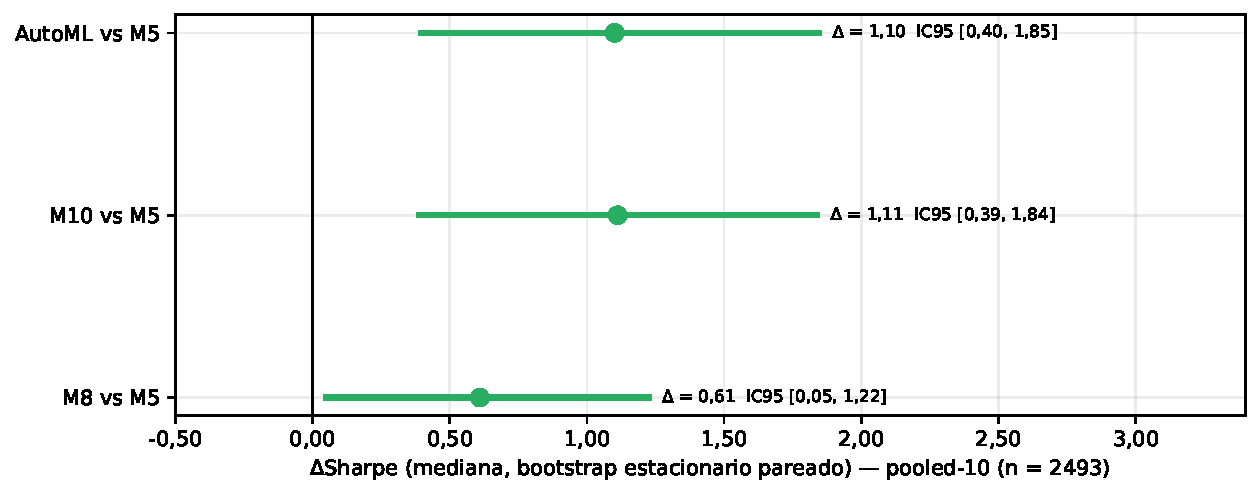
\includegraphics[width=0.60\textwidth]{figuras/cap4_forest_pooled}
\caption{Diagrama de bosque del $\Delta$Sharpe \emph{pooled-10} frente al agente M5, con intervalo al $95\%$ (\emph{bootstrap} estacionario, Politis y Romano 1994). La línea vertical marca el cero. Los tres intervalos excluyen el cero; la regla M8 con el límite inferior más cerca del borde y los aprendices M10 y AutoML con más holgura.}
\label{fig:mp-forest}
\end{figure}

El agregado tiene un matiz. El \emph{pooled} apila los días de los diez activos como si fueran independientes, y no lo son: la correlación cruzada entre índices es alta (SPY y QQQ por encima de $0{,}9$), lo que reduce el tamaño de muestra efectivo y deja el intervalo algo optimista. El bloque medio $\sqrt{n}$ del \emph{bootstrap} amortigua parte del efecto al remuestrear bloques contiguos.

En la economía, una derivada de STRATA bate al pasivo en Sharpe en cuatro activos: SPY, SMCI, MARA y UNG (Figura~\ref{fig:mp-equity-panel} del Anexo~\ref{anx:figuras}). En SMCI, MARA y UNG el pasivo pierde o ronda el cero y la derivada saca un Sharpe positivo yendo defensiva, sin estar largo en una subida. En SPY el periodo fue alcista y el activo es mayormente beta de mercado, así que el Sharpe positivo refleja sobre todo la exposición al índice.

\subsection{Equivalencia: el aprendiz redescubre STRATA y bate a la regla}
\label{sec:panel-tost}

Si el aprendiz mejora a la regla, ¿de qué se alimenta? Se apoya en los detectores de STRATA. Las cuotas de Shapley \cite{lundberg2017} miden cuánto del juicio del aprendiz descansa en cada bloque de características; la de las features de STRATA supera la mitad en los \textbf{diez de diez} activos, con una media de $0{,}66$. El aprendiz no inventa una señal nueva: redescubre los detectores que diseñamos a mano y los pondera por encima de las características del agente.

Que se apoye en STRATA no quiere decir que solo replique la regla. El contraste lo da el TOST de Schuirmann \cite{schuirmann1987}: al revés que un test de superioridad, parte de que las dos estrategias son distintas y solo concede equivalencia si la evidencia de parecido es fuerte, exigiendo rechazar por los dos lados a la vez. La Tabla~\ref{tab:mp-tost} lo aplica al aprendiz frente a la regla M8. En accuracy no hay equivalencia y el desempate va para el aprendiz: M10 y AutoML superan a la regla con un intervalo al $90\%$ por encima de cero. En Sharpe es no concluyente, indistinguibles en riesgo. El mecanismo es claro: la regla M8 es una compuerta fija sobre el régimen, mientras el aprendiz modela interacciones no lineales entre régimen y agente que la regla no alcanza, y de ahí saca el punto extra de accuracy.

\begin{table}[htbp]
\centering
\caption{TOST del aprendiz frente a la regla M8 (Schuirmann 1987) y cuota de Shapley de las features de STRATA por activo (Lundberg y Lee 2017). En accuracy el aprendiz supera a la regla (intervalo al $90\%$ por encima de cero); en Sharpe el test es no concluyente (indistinguibles). La cuota SHAP de STRATA supera $0{,}5$ en los diez activos.}
\label{tab:mp-tost}
\begin{tabular}{lccc}
\toprule
Comparación & $\Delta$accuracy (IC$_{90}$) & TOST Sharpe & Cuota SHAP STRATA \\
\midrule
M10 vs M8     & $+0{,}021\ [+0{,}001,\ +0{,}039]$ & no concluyente & \multirow{2}{*}{$>0{,}5$ en $10/10$ (media $0{,}66$)} \\
AutoML vs M8  & $+0{,}034\ [+0{,}010,\ +0{,}056]$ & no concluyente & \\
\bottomrule
\end{tabular}
\end{table}

El aprendiz deja, entonces, dos hechos atados con su test: se apoya en STRATA, con cuota SHAP mayoritaria en los diez activos, y bate modestamente a la regla en accuracy sin distinguirse de ella en riesgo (diagrama $2\times 2$ en la Figura~\ref{fig:mp-tost} del Anexo~\ref{anx:figuras}). La Tabla~\ref{tab:mp-capas} cierra el reparto sobre el panel (su lectura por detector, en la Figura~\ref{fig:mp-capas} del Anexo~\ref{anx:figuras}).

\begin{table}[htbp]
\centering
\caption{Atribución por capa sobre el panel de diez activos. La regla (M8) aporta el rescate de riesgo, con todo su P\&L de intervención concentrado en el canal de régimen (RAM, Figura~\ref{fig:mp-capas}); nunca lidera en accuracy. El aprendiz (M10/AutoML) aporta el rescate de accuracy y no lidera el riesgo en exclusiva. El capital final es sobre la ventana desplegable de SPY partiendo de un euro; el agente solo termina en $0{,}70\times$. $\Delta$Sharpe pooled frente al agente, IC$_{95}$ por bootstrap estacionario.}
\label{tab:mp-capas}
\begin{tabular}{lll}
\toprule
 & Regla (M8) & Aprendiz (M10/AutoML) \\
\midrule
Eje que rescata & riesgo & accuracy \\
$\Delta$Sharpe pooled vs M5 & $\mathbf{+0{,}60}$ $[0{,}05,\,1{,}22]$ & $+1{,}12$ / $+1{,}08$ \\
Capital final sobre SPY & $0{,}94\times$ & $0{,}92\times$ / $1{,}38\times$ \\
Lidera en accuracy & $0/10$ & $\mathbf{10/10}$ \\
Significancia accuracy (McNemar) & al borde & significativa \\
\bottomrule
\end{tabular}
\end{table}

\subsection{Complementariedad: bull, bear y diferencia en diferencias}
\label{sec:panel-regimen}

Un rescate que solo funcionara en mercado alcista no serviría de mucho, porque el régimen peligroso es el bajista. Partimos el panel por régimen y medimos el rescate en cada mitad con el McNemar pooled de la estrategia superior frente al agente, corrigiendo por Holm las comparaciones múltiples \cite{holm1979}. El rescate aparece en los dos (Tabla~\ref{tab:mp-regimen}): en alcista los dos aprendices rescatan de forma significativa y la regla M8 queda al borde; en bajista los tres pasan, con la regla ya holgadamente dentro.

\begin{table}[htbp]
\centering
\caption{Rescate por régimen (McNemar pooled de la estrategia superior frente a M5, $p$ corregido por Holm 1979) y complementariedad de los aprendices (DiD). El rescate es significativo en alcista y en bajista. El DiD contrasta el $\Delta\Delta$Sharpe entre aprendices y regímenes: M10 rescata más en alcista, AutoML más en bajista.}
\label{tab:mp-regimen}
\begin{tabular}{lccc}
\toprule
 & M8 & M10 & AutoML \\
\midrule
McNemar alcista (Holm $p$) & $0{,}099$ & $0{,}0076$ & $0{,}0092$ \\
McNemar bajista (Holm $p$) & $0{,}0092$ & $0{,}0268$ & $0{,}0017$ \\
\midrule
\multicolumn{4}{l}{DiD complementariedad: $\Delta\Delta$Sharpe pooled $= +1{,}37$, IC$_{95}\,[0{,}20,\ 2{,}60]$, $p = 0{,}008$} \\
\bottomrule
\end{tabular}
\end{table}

Los dos aprendices no rescatan igual en cada régimen: M10 protege más en alcista, AutoML más en bajista (Figura~\ref{fig:mp-did} del Anexo~\ref{anx:figuras}). Para contrastar si ese reparto es real construimos un test de diferencia en diferencias, pre-registrado: comparamos la diferencia de $\Delta$Sharpe entre los dos aprendices entre los dos regímenes, de modo que cualquier efecto común se cancela y queda solo la complementariedad. El $\Delta\Delta$Sharpe pooled excluye el cero (Tabla~\ref{tab:mp-regimen}): la complementariedad por régimen es significativa sobre el panel. El rescate en acierto también lo es en los dos regímenes (Figura~\ref{fig:anx-mcnemar}).

Queda la falsación pre-registrada, y el panel la resuelve. En SPY solo, en régimen bajista la regla M8 se invierte: sobre sus cincuenta días bajistas el $\Delta$Sharpe es $-1{,}49$, la regla daña en vez de rescatar. Sobre los diez activos el rescate por régimen es significativo en bajista, y la complementariedad DiD lo es en \emph{pooled} pero no en SPY aislado: el fenómeno es de panel. Queda el porqué del reparto por activo, y la respuesta está en la naturaleza del activo.

\section{El patrón: ley del leverage y clustering}
\label{sec:panel-patron}

% Clustering = EXPLORATORIO (n=10).

La sección anterior deja un hecho sin explicar: qué canal rescata cada activo cambia de uno a otro. La propiedad que ordena el rescate del aprendiz resulta ser el \emph{leverage effect}, y un clustering sin etiquetas recupera los mismos grupos que esa propiedad marca. Sobre diez activos esto es un patrón, no un teorema.

\subsection{La ley del \emph{leverage}}
\label{sec:panel-ley}

Los diez activos no son intercambiables (Figura~\ref{fig:mp-naturaleza} del Anexo~\ref{anx:figuras}): difieren en \emph{leverage}, en cuánta Crisis viven, en el sesgo del agente y en volatilidad.

El rescate del aprendiz en accuracy escala con el \emph{leverage effect} del activo. Medimos el rescate como $\max(\mathrm{M10},\mathrm{AutoML}) - \mathrm{M5}$ en accuracy y la naturaleza del activo con la correlación de Black, $\mathrm{leverage\_corr} = \operatorname{corr}(r_t,\ \mathrm{RV}^{21}_{t+1} - \mathrm{RV}^{21}_t)$, negativa cuando una caída eleva la volatilidad de mañana (\cite{black1976}; \cite{christie1982}).

Las dos magnitudes corren juntas: cuanto más negativo es el \emph{leverage} de un activo, más rescata el aprendiz en accuracy (Tabla~\ref{tab:mp-ley}, Figura~\ref{fig:mp-scatter}). La siguen nueve de los diez activos; ROKU es la única excepción, con \emph{leverage} casi nulo y un rescate alto. Hay un mecanismo detrás, el mismo de la Sección~\ref{sec:panel-pooled}: cuando el régimen es direccional, la regla disciplina el riesgo y al aprendiz le queda margen para afinar la dirección; cuando el régimen no informa el signo, el aprendiz rescata por otra vía y la ganancia se estrecha.

Con diez activos el contraste tiene poca potencia, de modo que lo presentamos como tendencia significativa al $\alpha = 0{,}10$ fijado por adelantado, no como ley exacta (Pearson $r = -0{,}56$, $p = 0{,}093$). Y su alcance es acotado: ordena el rescate del \emph{aprendiz}, no el de la regla, que no se deja predecir por la naturaleza del activo.

\begin{table}[htbp]
\centering
\caption{Ley del \emph{leverage}: correlación de Black y rescate del aprendiz por activo (panel de diez), ordenados por \emph{leverage} creciente. Rescate ${}= \max(\mathrm{M10},\mathrm{AutoML}) - \mathrm{M5}$ en accuracy. Nueve de los diez siguen la tendencia (a más \emph{leverage} negativo, más rescate); ROKU es la excepción. Sobre los diez: Pearson $r = -0{,}56$ ($p = 0{,}093$), Spearman $\rho = -0{,}59$ ($p = 0{,}074$); tendencia significativa al $\alpha = 0{,}10$ pre-registrado.}
\label{tab:mp-ley}
\begin{tabular}{lrrl}
\toprule
Activo & \texttt{leverage\_corr} & Rescate aprendiz & \\
\midrule
DIA  & $-0{,}112$ & $0{,}080$ & \\
SPY  & $-0{,}110$ & $0{,}207$ & \\
QQQ  & $-0{,}092$ & $0{,}116$ & \\
XLF  & $-0{,}091$ & $0{,}097$ & \\
XLE  & $-0{,}089$ & $0{,}085$ & \\
XLK  & $-0{,}086$ & $0{,}080$ & \\
MARA & $-0{,}059$ & $0{,}016$ & \\
SMCI & $-0{,}004$ & $0{,}068$ & \\
ROKU & $+0{,}003$ & $0{,}100$ & (excepción) \\
UNG  & $+0{,}041$ & $0{,}008$ & \\
\midrule
\emph{leverage} fuerte (media) & & $0{,}097$ & \\
\emph{leverage} débil (media)  & & $0{,}059$ & \\
\bottomrule
\end{tabular}
\end{table}

\begin{figure}[htbp]
\centering
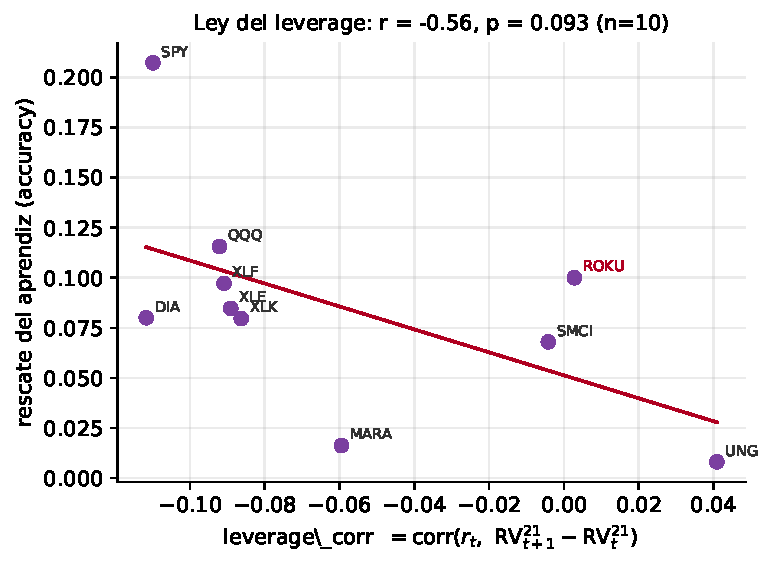
\includegraphics[width=0.60\textwidth]{figuras/cap4_scatter_leverage}
\caption{Rescate del aprendiz en accuracy frente al \emph{leverage} del activo, sobre los diez. Cada punto es un activo; el eje horizontal es la correlación de Black $\operatorname{corr}(r_t,\ \mathrm{RV}^{21}_{t+1}-\mathrm{RV}^{21}_t)$, el vertical el rescate $\max(\mathrm{M10},\mathrm{AutoML}) - \mathrm{M5}$. La recta de regresión baja con el \emph{leverage}: a más \emph{leverage} negativo, más rescate (Pearson $r = -0{,}56$, $p = 0{,}093$; tendencia significativa al $\alpha = 0{,}10$ pre-registrado). Nueve de los diez la siguen; ROKU, señalado, es la excepción.}
\label{fig:mp-scatter}
\end{figure}

\subsection{Clustering: la naturaleza separa los grupos}
\label{sec:panel-clustering}

La ley del \emph{leverage} es una recta. Queda ver si la misma estructura aparece cuando no le decimos al algoritmo qué buscar. Aparece: describimos cada activo por cinco rasgos de naturaleza (\emph{leverage}, retorno medio en Crisis, fracción de días en Crisis, volatilidad OOS y sesgo direccional del agente) y lo agrupamos con cuatro métodos —$k$-medias \cite{macqueen1967,lloyd1982}, enlace de Ward \cite{ward1963}, mezcla gaussiana \cite{dempster1977} y clustering espectral \cite{ng2002spectral}— sin ver ni una métrica de rescate.

Los cuatro coinciden en una partición unánime y bien separada (Tabla~\ref{tab:mp-cluster}): con tres grupos, el índice de Rand ajustado entre cualquier par de métodos vale uno \cite{hubert1985}. Cada grupo trae asociado un canal de rescate distinto: los índices de \emph{leverage} fuerte y los volátiles, rescatados por AutoML, y los de \emph{leverage} invertido, por M10. Los perfiles de accuracy y Sharpe por grupo están en la Figura~\ref{fig:anx-grupos}.

El cierre lo da la geometría. Al proyectar la naturaleza de los diez sobre sus dos primeras componentes principales, el primer eje recupera casi exactamente el \emph{leverage} ($r = 0{,}84$ entre PC1 y \texttt{leverage\_corr}, Figura~\ref{fig:mp-pca}): sin etiquetas de rescate, el clustering ordena los activos por el mismo eje que la ley de la Sección~\ref{sec:panel-ley}. La Figura~\ref{fig:mp-casos} del Anexo~\ref{anx:figuras} lo aterriza en dos casos, XLE rescatado por el régimen y MARA por la vía del \emph{leverage} invertido.

Con diez activos esto es exploratorio: el clustering describe, no confirma. El cluster predice el \emph{tipo} de canal que rescata cada grupo, no el modelo exacto que ganará por activo, que puede cambiar dentro de un mismo grupo. Se deja para líneas futuras.

\begin{table}[htbp]
\centering
\caption{Perfil de los tres grupos del \emph{clustering} de la naturaleza de los diez activos (cinco rasgos: \emph{leverage}, retorno medio en Crisis, fracción en Crisis, volatilidad OOS, sesgo del agente): \emph{leverage} medio de cada grupo y su mejor canal de rescate. Los cuatro métodos coinciden en esta misma partición (Rand $= 1{,}0$, silueta $0{,}55$).}
\label{tab:mp-cluster}
\begin{tabular}{lrl}
\toprule
Cluster & \emph{leverage} medio & Mejor canal \\
\midrule
C0 índices (SPY, QQQ, XLF, DIA, XLK, XLE) & $-0{,}097$ & AutoML \\
C1 \emph{leverage} invertido (SMCI, UNG)  & $+0{,}018$ & M10 \\
C2 volátiles (ROKU, MARA)                 & $-0{,}028$ & AutoML \\
\bottomrule
\end{tabular}
\end{table}

\begin{figure}[htbp]
\centering
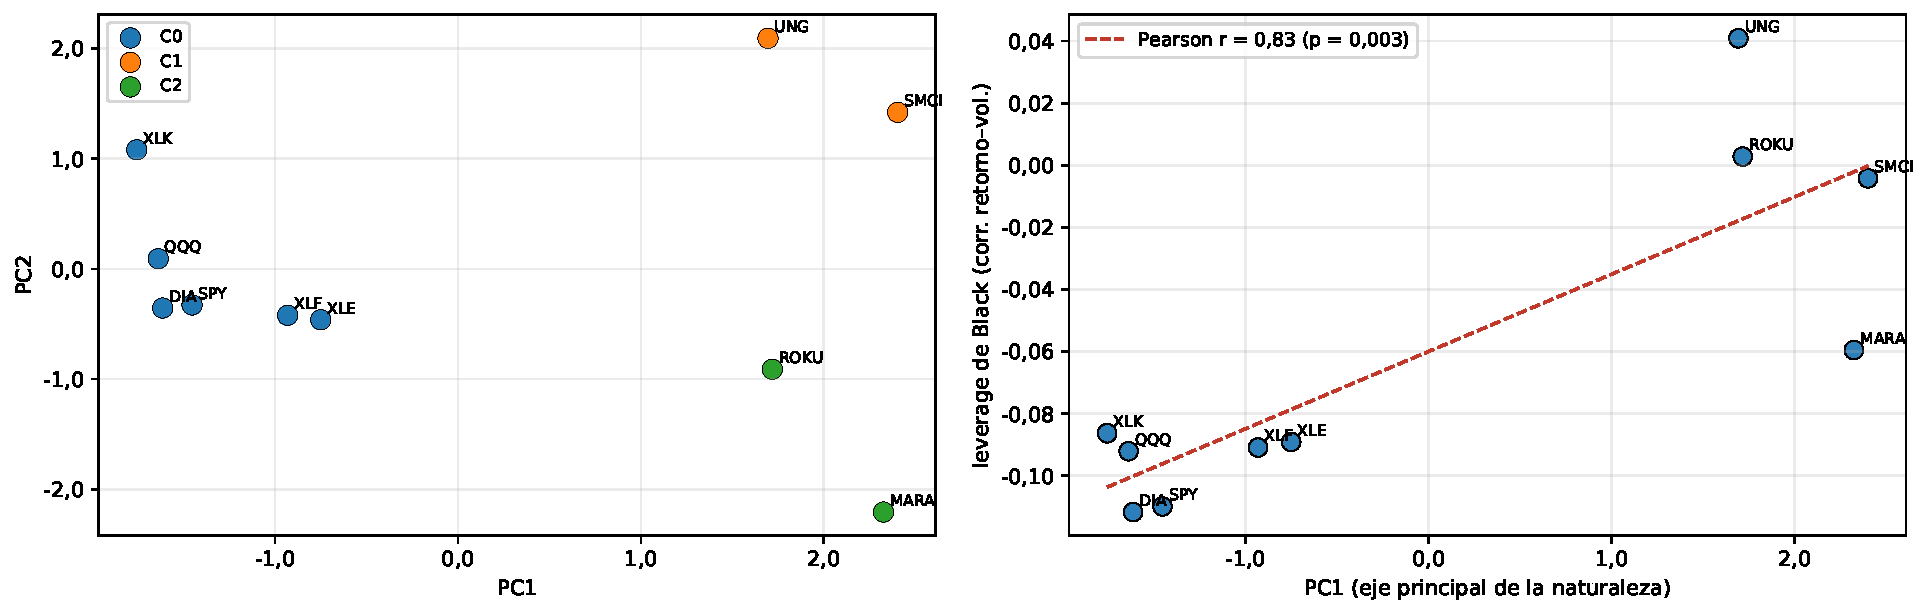
\includegraphics[width=0.60\textwidth]{figuras/cap4_pca_clusters}
\caption{Proyección de la naturaleza de los diez activos sobre sus dos primeras componentes principales. Cada punto es un activo, coloreado por su cluster ($K=3$, partición unánime de los cuatro métodos, Rand $= 1{,}0$). El primer eje recupera el \emph{leverage} ($r = 0{,}84$ entre PC1 y \texttt{leverage\_corr}): el clustering ordena los activos, sin etiquetas de rescate, por el mismo eje que la ley del \emph{leverage}. La leyenda marca el mejor canal de cada grupo (C0/C2 AutoML, C1 M10).}
\label{fig:mp-pca}
\end{figure}

\section{Robustez}
\label{sec:panel-robustez}

El rescate no depende de una elección afortunada. Se mantiene al mover la ventana de calibración de los detectores (Figura~\ref{fig:mp-robustez-calib} del Anexo~\ref{anx:figuras}) y aguanta en el panel por tres vías a la vez: la importancia de STRATA es estable en el tiempo, el rescate sobrevive a distintas particiones y se sostiene partido por régimen (Figura~\ref{fig:mp-robustez-panel} del Anexo~\ref{anx:figuras}).

\section{Alcance y limitaciones}
\label{sec:panel-limites}
\label{sec:panel-lim-tests}

Cuatro resultados del capítulo viven por debajo del listón de la significancia. La Tabla~\ref{tab:mp-limites} los reúne con su contraste y su veredicto. El que más pesa: la victoria sobre la trivial es nominal. La regla, además, se invierte en SPY-bajista, una falsación que pre-registramos y que la agregación del panel resuelve.

\begin{table}[htbp]
\centering
\caption{Resumen de los resultados que no alcanzan significancia plena, con su contraste y su veredicto. La columna de veredicto distingue lo nominal de lo falsado y de lo exploratorio.}
\label{tab:mp-limites}
\begin{tabular}{p{4.4cm}p{4.6cm}p{4.0cm}}
\toprule
Afirmación & Test y cifra & Veredicto \\
\midrule
Una derivada bate a la trivial en accuracy & McNemar AutoML vs ZeroR sobre SPY, $p = 0{,}902$ & Nominal ($n \approx 250$, a posteriori) \\
\addlinespace
El rescate en accuracy escala con el \emph{leverage} & Pearson $r = -0{,}56$, $p = 0{,}093$; Spearman $\rho = -0{,}59$, $p = 0{,}074$ (diez activos) & Tendencia al $\alpha = 0{,}10$; no $p < 0{,}05$ \\
\addlinespace
La regla M8 rescata el riesgo en SPY-bajista & $\Delta$Sharpe $= -1{,}49$ ($n = 50$) & Falsación pre-registrada, resuelta por el panel \\
\addlinespace
La naturaleza define grupos de activos & Consenso de cuatro métodos, Rand $= 1{,}0$ (diez activos) & Exploratorio, no predictivo por activo \\
\bottomrule
\end{tabular}
\end{table}

El límite común es la ventana corta: con $n \approx 250$ días, la significancia plena frente a la trivial está fuera de alcance por potencia, no por ausencia de señal. La pregunta con la que abrimos queda respondida: lo que en SPY no alcanzaba significancia en solitario la alcanza al agregar.
